\section{Poisson-Boltzmann Equation}
We are considering the Poisson-Boltzmann Equation (PBE) as the governing equation for a solute macro molecule immersed in an aqueous solvent environment illustrated in Figure \ref{fig_PBmodel} (a). Our computational domain $\Omega \in \mathbb{R}^3$ is separated into two regions $\Omega^-$ and $\Omega^+$ by the molecular surface $\Gamma$, which is an arbitrarily shaped dielectric interface. Here $\Omega^-$ is the molecular region with dielectric constant $\epsilon^-$ and $\Omega^+$ is the solvent region with dielectric constant $\epsilon^+$. The cubic shape boundary of $\Omega= \Omega^-\cup \Omega^+ $ is denoted by $\partial \Omega$. The charges at the center of each atom inside $\Gamma$, have been distributed as the partial charges to the nearest grid points by the Trilinear interpolation as shown in Figure \ref{fig_PBmodel} (b). The charges outside $\Gamma$ are actually mobile ions which are described by the Boltzmann distribution. 

\begin{figure}[t]
\centering
	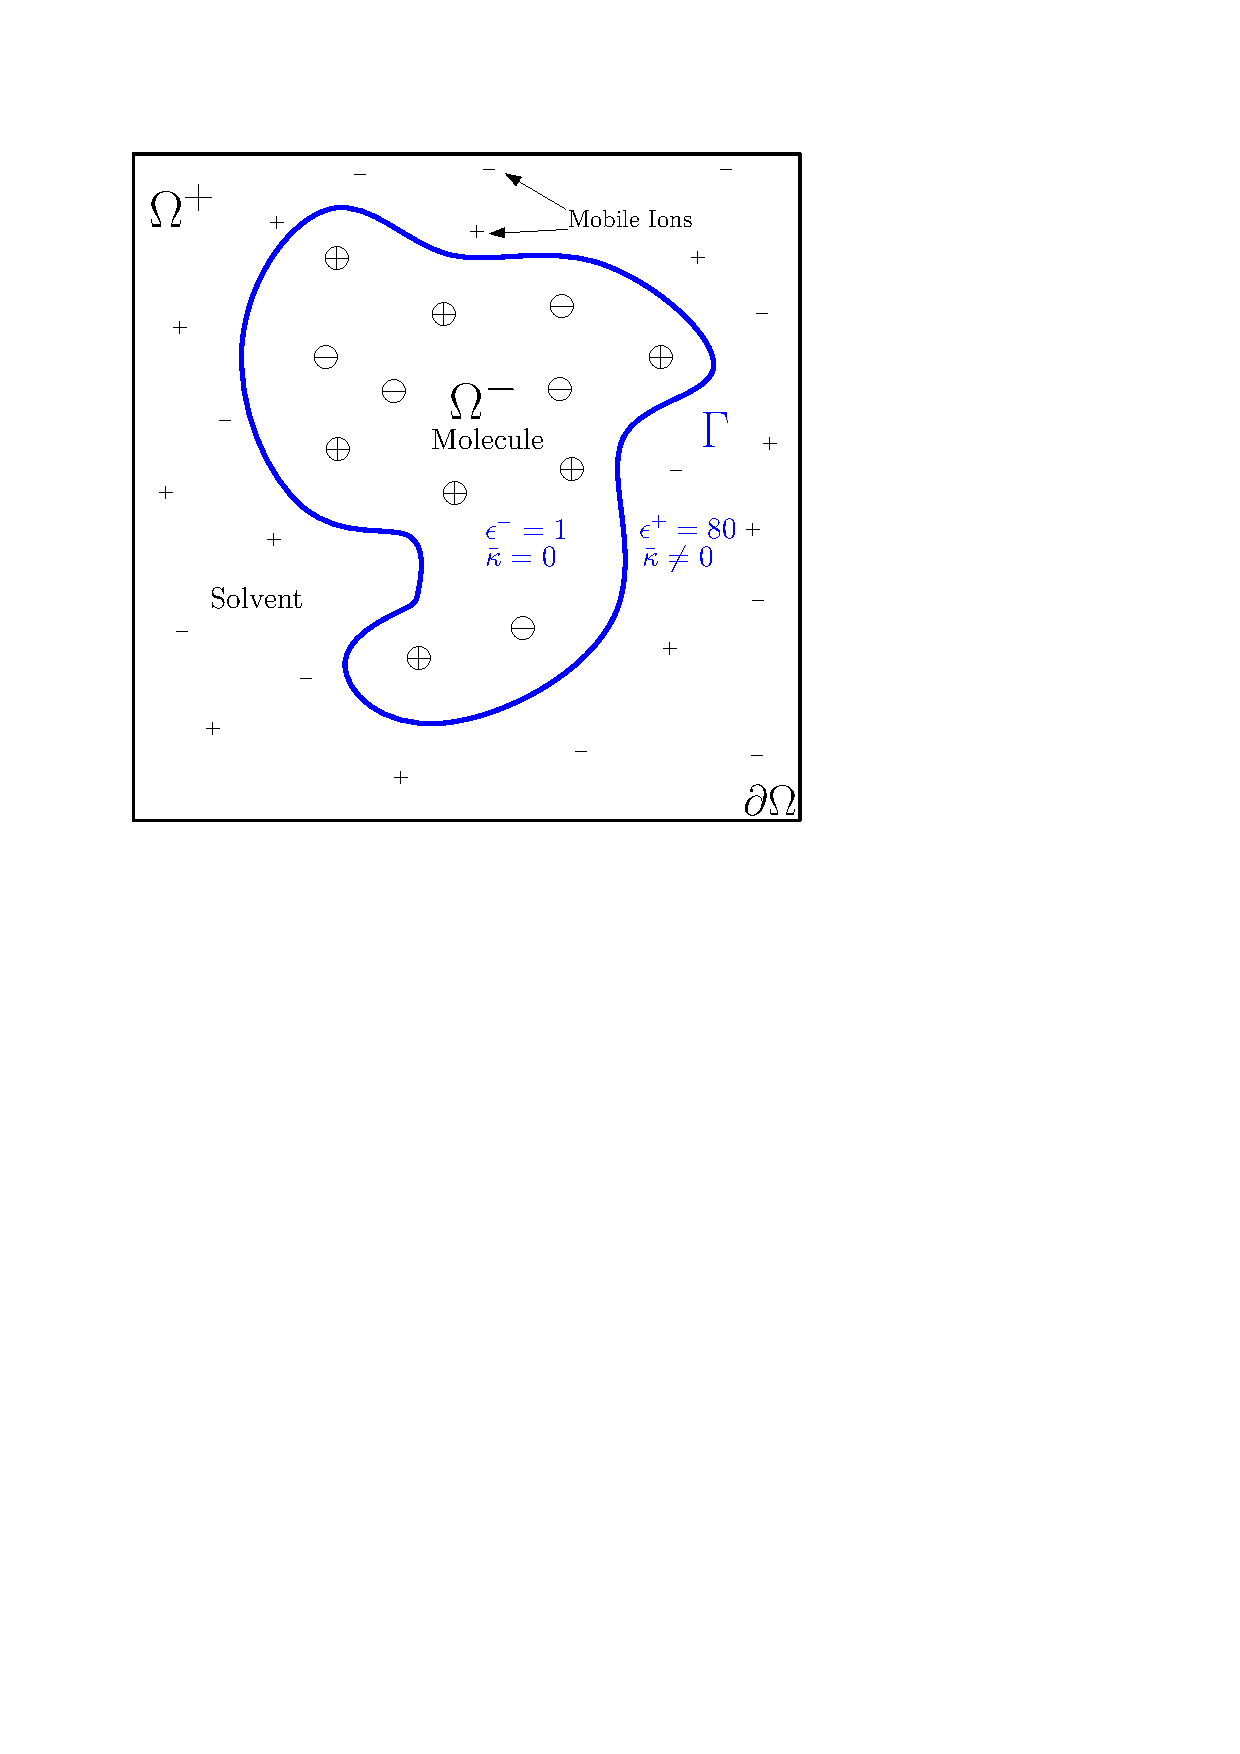
\includegraphics[width =0.4\textwidth]{PBE_domain.pdf}
	\hspace{8mm}
	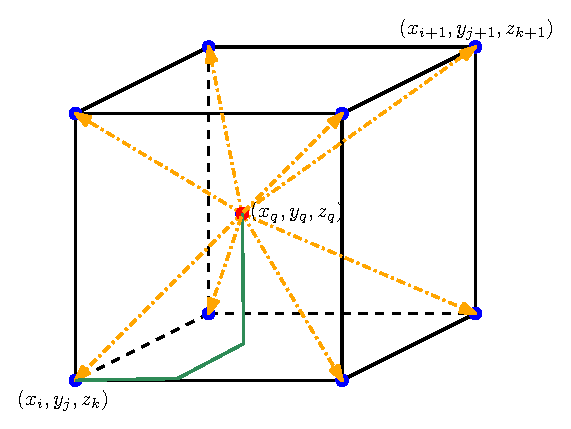
\includegraphics[width =0.5\textwidth]{chg_dist.eps}\\
	(a)\hspace{3.3in}(b)
	\caption{(a) Poisson-Boltzmann Model. (b) Charge $q$ (red) is distributed to 8 grid points (blue).}
	\label{fig_PBmodel}
\end{figure}
%\begin{figure}[!h]
%	\centering
%	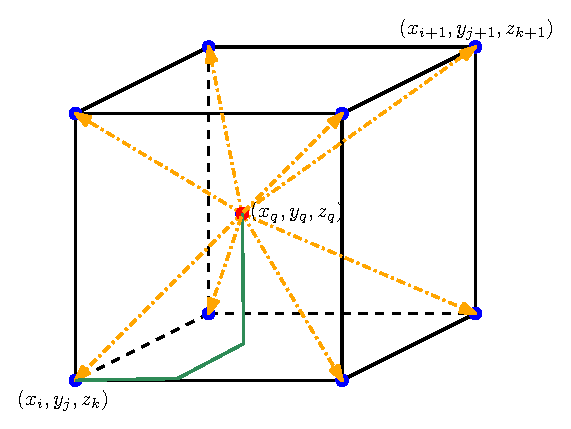
\includegraphics[width = 0.7\textwidth]{chg_dist.eps}
%	\caption{Charge $q$ (red) is distributed to 8 grid points (blue).}
%	\label{fig:chg_dist}
%\end{figure}

The electrostatic interaction of this solute-solvent system for $\textbf{r} \in \mathbb{R}^3$ is governed by the nonlinear Poisson-Boltzmann Equation (PBE) as, 
\begin{equation}
			-\nabla.(\epsilon(\textbf{r})\nabla \phi(\textbf{r}))+\bar\kappa^2(\textbf{r}) \sinh (\phi(\textbf{r}))=\rho(\textbf{r}).\label{pbe} %\\
					%\left[\phi \right]_\Gamma = 0 \textnormal{ and } \left[\epsilon\phi_n\right]_\Gamma = 0 
\end{equation}
We have used the following approximated analytical solution \cite{Holst1995} as the boundary condition
\begin{equation}
	\phi_b (\textbf{r}) = \frac{e_c^2}{k_B T} \sum_{i=1}^{N_c} \frac{q_i e^{-|\textbf{r}-\textbf{r}_i | \sqrt{\frac{\bar\kappa^2}{\epsilon^+}} }}{\epsilon^{+}|\textbf{r}-\textbf{r}_i|}, \label{bd_cond}
\end{equation}
where the singular source $\rho(\textbf{r})$ term is defined as,
\begin{equation}
	\rho(\textbf{r})= 4\pi \frac{e_c^2}{k_B T}\sum_{i=1}^{N_c} q_i \delta(\textbf{r}-\textbf{r}_i). \label{rho}
\end{equation}

Here $N_c$ is the total number of atoms in the solute molecule, $k_B$ is the Boltzmann constant, $e_c$ is the fundamental charge and $q_i$, in the same unit as $e_c$ is the partial charge on the \textit{i}th atom of the solute molecule located at position $\textbf{r}_j$. The Debye-Huckel parameter $\bar\kappa^2 =\Big(\frac{2N_A e_c^2}{100 k_b T}\Big)I_s =  8.486902807$\AA$^{-2} I_s$ from \cite{Holst:1993} for $\textbf{r} \in \Omega^+$ and $\bar\kappa=0$ for $\textbf{r} \in \Omega^-$. Here $N_A$ is  the Avogadro’s Number and $I_s$ is the molar ionic strength. We have converted the dimensionless electrostatic potential $u$ to the units kcal/mol/$e_c$ at the room temperature $T$ by multiplying it by $0.592183$ \cite{Holst:1993}. There are two conditions on $\Gamma$ needed to be satisfied from the dielectric theory for the potential $\phi$ and flux density $\epsilon \phi_\textbf{n} $, 
\begin{equation}
\left[\phi \right]_\Gamma = 0 \textnormal{ and } \left[\epsilon\phi_n\right]_\Gamma = 0. \label{ju_cond}
\end{equation}
where $\textbf{n}=(n_x,n_y,n_z)$ is the outer normal direction on the interface $\Gamma$ and $\phi_\textbf{n}= \frac{\partial \phi}{\partial\textbf{n}} $ is the directional derivative in \textbf{n}. The notation $[f]_\Gamma = f^+-f^-$ represents the difference of the functional value across the interface $\Gamma$. The dielectric constant $\epsilon$ is a piecewise constant such that, $\epsilon(\textbf{r})=\epsilon^-$ for $\textbf{r} \in \Omega^-$ and $\epsilon(\textbf{r})=\epsilon^+$ for $\textbf{r} \in \Omega^+$. 

%The reader can refer to REF1 and REF2 for more details about definitions and units of these coefficients. 
%%%%%%%%%%%%%%%%%%%%%%%%%%%%%%%%%%%%%%%%%%%%%%%%%%%%%%%%%%%%%%%%%%%%%%%%%%%%%
\section{Molecular surfaces}
\label{sec:m_srface}
A Molecular surface plays an important role to solve the PBE equation by setting the interface between $\Omega^-$ and $\Omega^+$. The location of the centers of the atoms in a molecule and their Van der Waals radius have been used to construct the following types of molecular surface in the literature.  
\begin{figure}[!t]
	\begin{center}
		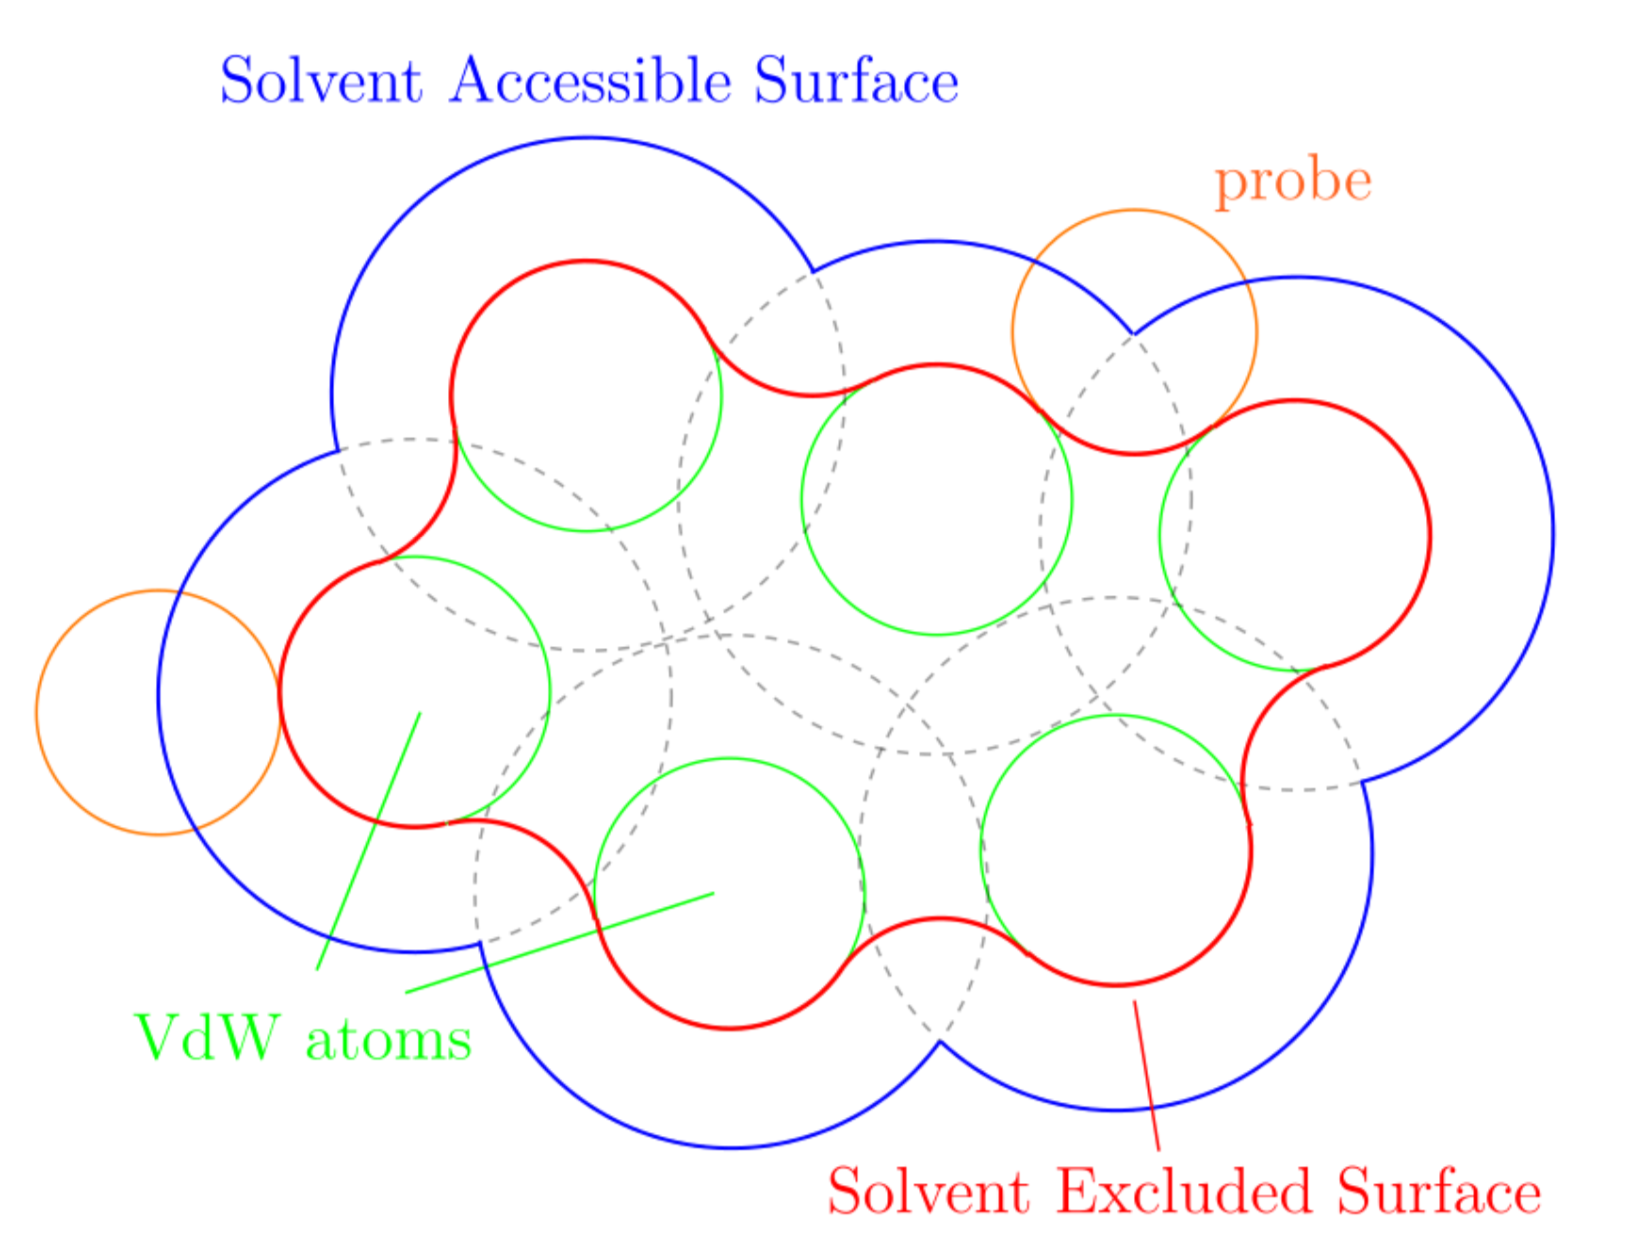
\includegraphics[scale = 0.3]{M_surface.png}
	\end{center}
	\caption{2D diagram of the Van der Waals (VdW) Surface (green), Solvent Accessible Surface
(SAS) (blue), Solvent Excluded Surface (SES) (red) \cite{Quan2018}.}
\label{fig:M_surface}
\end{figure}

{\bf Van der Waals (VdW) surface}: The simplest type of molecular surface can be thought of a union of atomic spheres known as Van der Waals balls using their Van der Waals radius. The surface generated by this process is called as Van der Waals (VdW) Surface as shown in Figure \ref{fig:M_surface}. These types of surfaces are often not suitable for PB models due to their singularities at the intersections of the spheres.  

{\bf SAS and SES surfaces:} Two other kinds of molecular surfaces that are commonly used for PB models are the Solvent Accessible Surface (SAS) and the Solvent Excluded Surface (SES) introduced by Lee and Richards in 1970's \cite{LEE1971379,Fred1977}. In their approach, the solvent molecules surrounding a solute molecule are reduced to spherical probes \cite{Tomasi2005}. The SAS is defined as the path of the center of the solvent probe when it roles over the solute molecule. That is, SAS is the surface enclosing the region in which the {\it center} of the solvent probe cannot enter. On the other hand, SES is defined as the surface enclosing the region in which the {\it surface} of the solvent probe can not enter. The SAS surface might have the same type of singularity but SES is known for its smoothness and called “the smooth molecular surface” or “the Connolly surface”, due to Connolly’s fundamental work \cite{Connolly1983}. Besides these sharp interfaces, other soft interfaces like the Gaussian interface have been considered for PBE \cite{Hazra2019}.   
\begin{figure}[!t]
	\centering
	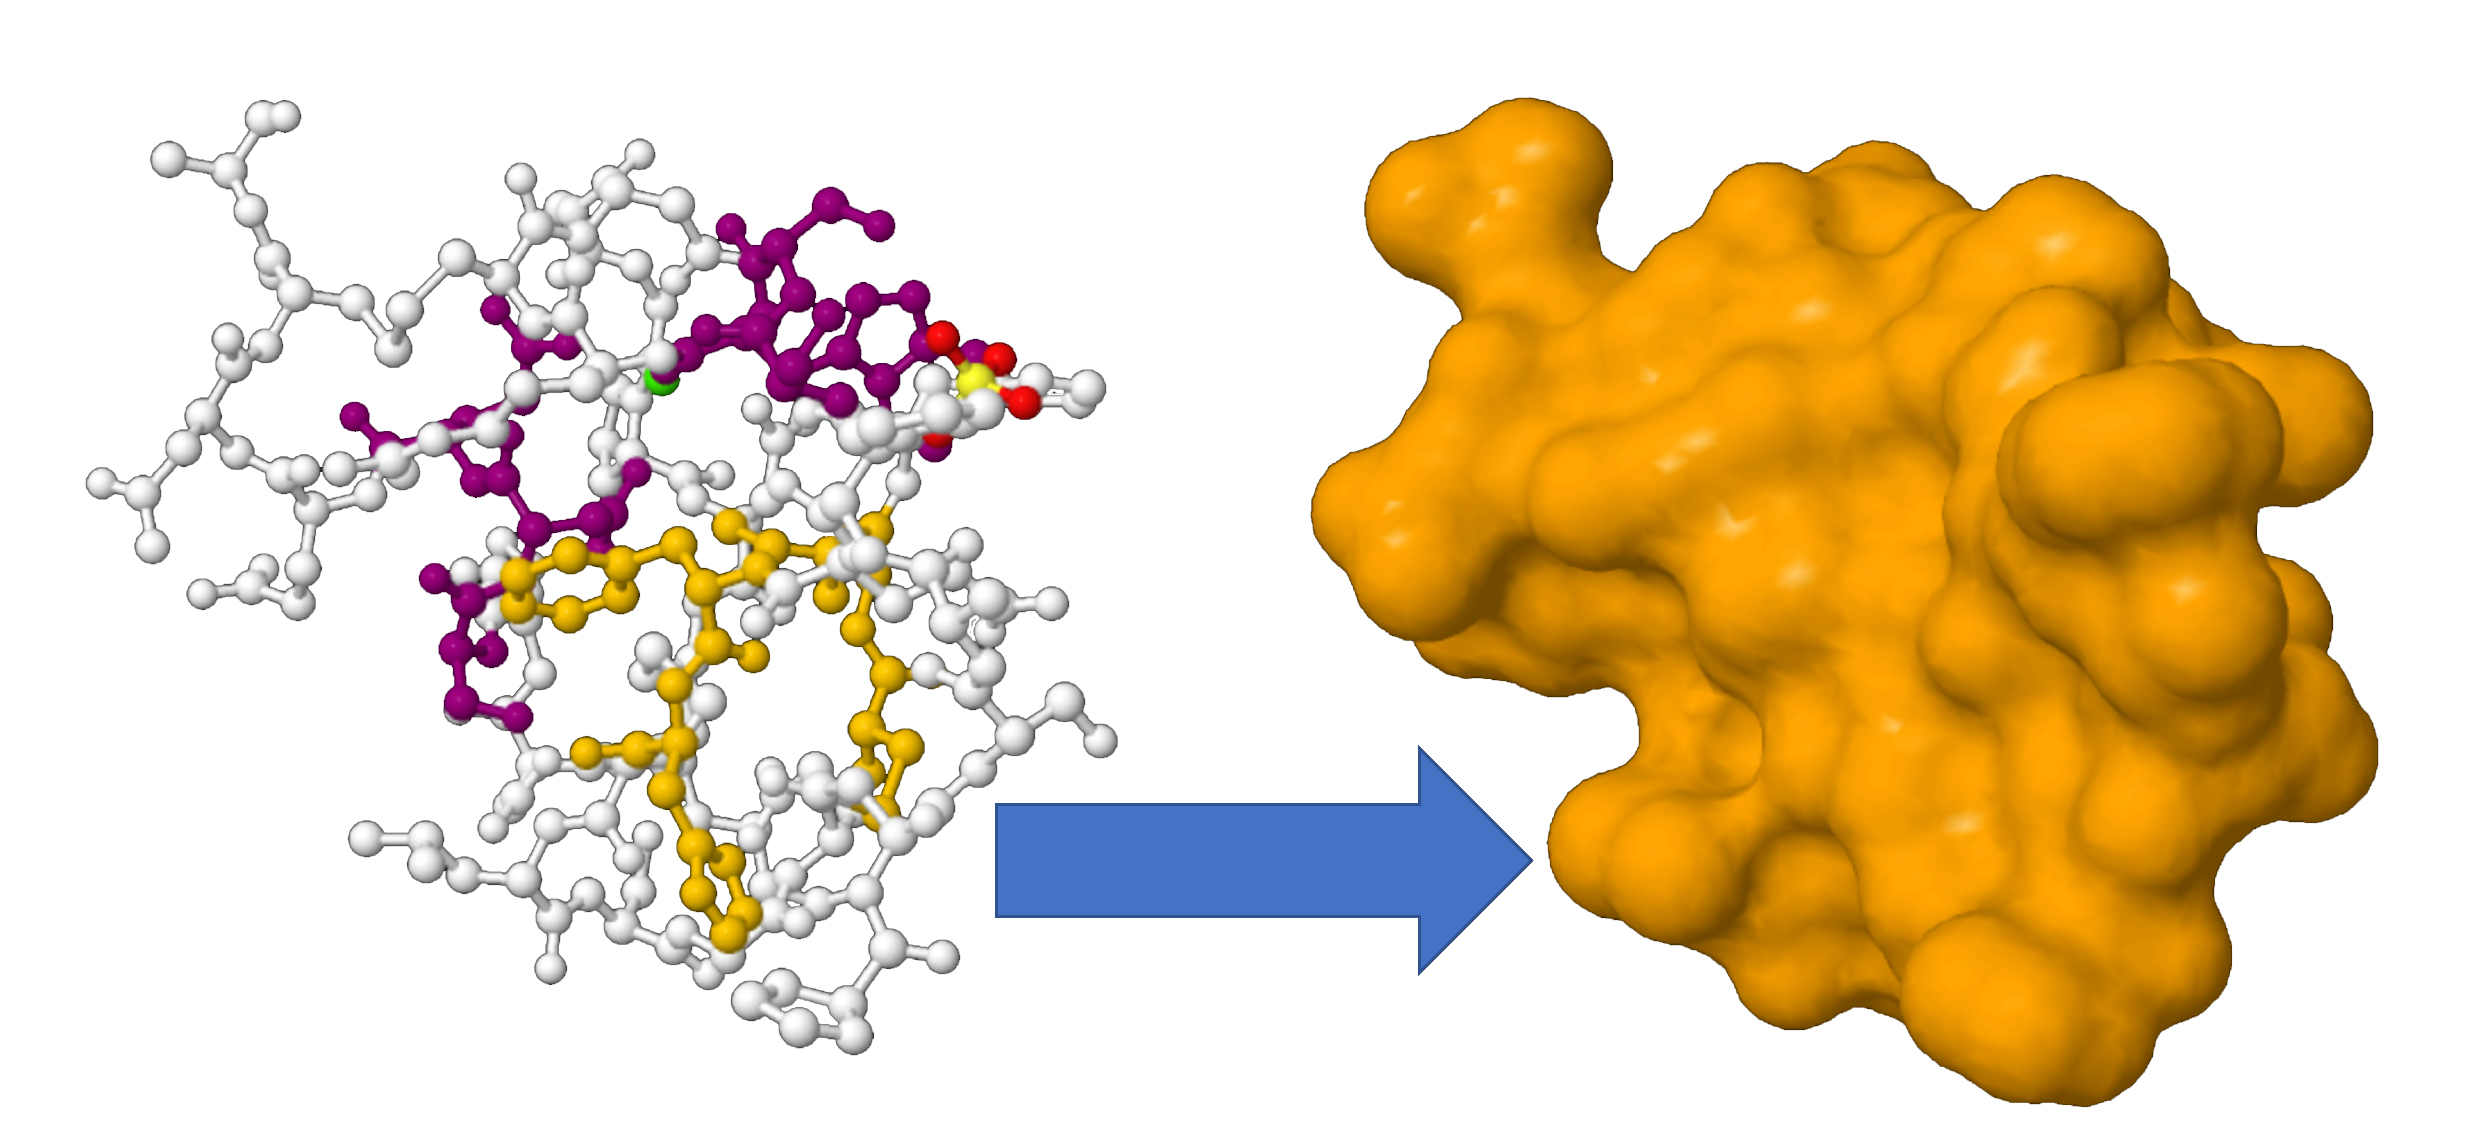
\includegraphics[scale  = .35]{1ajj_surface_white.jpg}	
	\caption{Molecular Surface of the protein \textit{1ajj} generated by MSMS}
	\label{fig:1ajj_surface}
\end{figure}

For our computations we used the {\it reduced surface} developed by Sanner and his team  \cite{MSMS} at the Molecular Graphics Laboratory (TSRI) along with the MSMS (Michel Sanner’s Molecular Surface) algorithm for computing an approximate analytical representation of the SES. It uses the input files for the ADI-MSMS package and produces two files with extensions {\it .vert} and {\it .face}. Later these output files from the MSMS package are used to create the molecular surface as shown in Figure \ref{fig:1ajj_surface} to decide whether a grid point is inside or outside the solute molecule. 

%%%%%%%%%%%%%%%%%%%%%%%%%%%%%%%%%%%%%%%%%%%%%%%%%%%%%%%%%%%%%%%%%%%%%%%%%%%%%

\section{ADI Method for pseudo transient PBE}
\label{sec:adi-method}

The pseudo-transient variation to the PBE has become popular approach for solving the nonlinear PBE \cite{Sayyed-Ahmad2004, Shestakov2002, Zhao2011, zhao_operator_2014}. In this approach equation (\ref{pbe}) is converted to the following time dependent PBE (TPBE),

\begin{equation}
			\frac{\partial \phi(\textbf{r},t)}{\partial t}=\nabla.(\epsilon(\textbf{r})\nabla \phi(\textbf{r},t))-\bar\kappa^2(\textbf{r}) \sinh (\phi(\textbf{r},t))+\rho(\textbf{r}).\label{eq:tpbe} %\\
					%\left[\phi \right]_\Gamma = 0 \textnormal{ and } \left[\epsilon\phi_n\right]_\Gamma = 0 
\end{equation}
%In \cite{Geng2013_Fully} equation (\ref{eq:tpbe}) has later been separated in two separate equation using a first order time splitting like equation (\ref{eq:non_linear_ADI}) and (\ref{eq:diffusion_ADI}) in section \ref{sec:GFM-ADI}. Then the nonlinear equation has been solved by an analytical solution and the Douglas-Rachford ADI scheme has been used for the other diffusion equation. But in terms of intrer


Here only $\phi$ is time dependent, while all other functions in (\ref{eq:tpbe}), i.e. $\epsilon,\rho$ and $\bar\kappa^2 $ are time independent. Let us consider a uniform mesh with a grid spacing $h$ in all $x,y$ and $z$ directions having $N_x,N_y$ and $N_z$ as the number of the grid points in each direction. We assume the vector ${{\bf U}^n = \phi^n_{ijk}}$ for $i=1,...., N_x,j=1,...,$ and $N_y,k=1,...N_z$ denote all the nodal values of $\phi$ at the time level $t_n$. Two stages of operator splitting schemes are used for updating $\phi^n$ at time level $t_n$ to $\phi^{n+1}$ at time level $t_{n+1}=t_n+ \Delta t $. 


At the first stage, equation (\ref{eq:tpbe}) is separated into the following two equations using a first order time splitting,
\begin{eqnarray}
  \frac{\partial w}{\partial t}&=& -\bar\kappa^2 \sinh(w) \text{ with } {\bf W}^n={\bf U}^n\text{ and } t \in \left[t_n,t_{n+1}\right],\label{eq_nonl_ADI1}\\
 \frac{\partial v}{\partial t}&=&  \nabla . (\epsilon\nabla v)+\rho({\bf r}) \text{ with } {\bf V}^n={\bf W}^{n+1}\text{ and } t \in \left[t_n,t_{n+1}\right],	 \label{eq_diff_ADI1}
\end{eqnarray}
where ${\bf U}^{n+1}={\bf V}^{n+1}$. Equation (\ref{eq_nonl_ADI1}) has the following analytical solution (\ref{eq:anal_sol}) in \cite{Geng2013_Fully},
	\begin{eqnarray}	
{\bf W}^{n+1}= \ln \left( \frac{\cosh(\frac{1}{2}\bar\kappa^2\Delta t)+\exp(-{\bf W}^n)\sinh(\frac{1}{2}\bar\kappa^2\Delta t)}{\exp(-{\bf W}^n)\cosh(\frac{1}{2}\bar\kappa^2\Delta t)+\sinh(\frac{1}{2}\bar\kappa^2\Delta t)}\right).\label{eq:anal_sol}
\end{eqnarray}
This is helpful to avoid the difficulty due to the nonlinear $\sinh()$ term in (\ref{pbe}). The right hand side of equation (\ref{eq:anal_sol}) is just a function of $W^n$ and $\Delta t$ so that ${\bf W}^{n+1}=F({\bf W}^n,\Delta t)$. Then for the discretization of equation (\ref{eq_diff_ADI1}), Backward-Euler integration in time and central differencing in space results in, 
\begin{eqnarray}
	v_{i,j,k}^{n+1} &=v_{i,j,k}^{n}+\Delta t \left(\Delta_x^2+\Delta_y^2+\Delta_z^2\right)v_{i,j,k}^{n+1}+\Delta t \rho({\bf r}), \label{eq:imp_ADI}
\end{eqnarray}
where $\Delta_x,\Delta_y$ and $\Delta_z$ are the central finite difference operators in $x,y$ and $z$ directions defined as, 
  \begin{eqnarray}
% \begin{aligned}
% \begin{equation}
	\Delta_x^2\left(v_{i,j,k}^n\right)&=& \frac{1}{h^2} \left(\epsilon_{i+\frac{1}{2},j,k}(v_{i+1,j,k}^n-v_{i,j,k}^n)+\epsilon_{i-\frac{1}{2},j,k}(v_{i-1,j,k}^n-v_{i,j,k}^n)\right), \nonumber \\
	\Delta_y^2\left(v_{i,j,k}^n\right)&=& \frac{1}{h^2} \left(\epsilon_{i,j+\frac{1}{2},k}(v_{i,j+1,k}^n-v_{i,j,k}^n)+\epsilon_{i,j-\frac{1}{2},k}(v_{i,j-1,k}^n-v_{i,j,k}^n)\right),\\ \label{eq:dif_opx_adi1}
	\Delta_z^2\left(v_{i,j,k}^n\right)&=&\frac{1}{h^2} \left(\epsilon_{i,j,k+\frac{1}{2}}(v_{i,j,k+1}^n-v_{i,j,k}^n)+\epsilon_{i,j,k-\frac{1}{2}}(v_{i,j,k-1}^n-v_{i,j,k}^n)\right).  \nonumber
%\end{equation}	
%	\end{aligned}
\end{eqnarray}
Here the $\epsilon$-halves ($\epsilon_{i+\frac{1}{2},j,k},\epsilon_{i,j+\frac{1}{2},k}$ and $\epsilon_{i,j,k+\frac{1}{2}}$) are the average of the dielectric constants value at two adjacent grid point in $x,y$ and $z$ directions. 

For the second stage in the operator splitting, the following Douglas-Rachford type ADI scheme is then introduced for the equation (\ref{eq:imp_ADI})\cite{Geng2013_Fully}.   
\begin{eqnarray}
%\begin{aligned}
		\left(1- \Delta t \Delta_x^2\right)v_{i,j,k}^{*}&=&\left[1+ \Delta t \left(\Delta_y^2+\Delta_z^2 \right)\right]v_{i,j,k}^{n}+\Delta t \rho({\bf r}),\label{eq_ADI1}\nonumber \\ 
		\left(1-\Delta t \Delta_y^2\right)v_{i,j,k}^{**}&=&v_{i,j,k}^{*}- \Delta t \Delta_y^2\left(v_{i,j,k}^{n}\right),\label{GFM-ADI2}\\
		\left(1- \Delta t \Delta_z^2\right)v_{i,j,k}^{n+1}&=&v_{i,j,k}^{**}- \Delta t \Delta_z^2\left(v_{i,j,k}^{n}\right).\label{GFM-ADI3}\nonumber
%\end{aligned}		\label{1dadi}
\end{eqnarray}
The ADI method discussed in \cite{Geng2013_Fully} is a promising tool to solve the nonlinear PBE but it does not focus on the issues due to the singularity at the source terms and the jump conditions on the interface. As we will observe in Chapter \ref{chap:num_vald}, these two issues reduce the accuracy and stability of the ADI method significantly.  
       
%%%%%%%%%%%%%%%%%%%%%%%%%%%%%%%%%%%%%%%%%%%%%%%%%%%%%%%%%%%%%%%%%%%%%%%%%%%%%


\section{Cleaning ADI-MSMS package to develop REG-GFM-MSMS package}	
To simulate the ADI Methods in \cite{Geng2013_Fully} and the LOD Methods in \cite{Wilson2016}, Dr. Shan Zhao and Dr. Weihua Geng from the Southern Methodist University developed a coding package named ADI-MSMS. This package uses two types of protein data files for a particular protein as inputs and calculates the electrostatic potential $\phi$ and the solvation energy as the outputs. The input files are generated from the {\it .pdb} and {\it .pqr } file. This package uses a sub-package called  FISHPACK90 which was originally developed by the NCAR (National Center for Atmospheric Research) back in the late 70's and revised later in 90's. It is a collection of FORTRAN programs and subroutines that solve second-order and fourth-order finite difference approximations to  the elliptic partial differential equations. The ADI-MSMS package has also been used to solve the Poisson Equation for a special case of the PBE when the protein molecule is in a vacuum instead of being surrounded by the solvent.
%	\item {\bf MSMS:} It is a program \cite{MSMS} written in the programming language C to compute the molecular surface. It was developed by  Michel Sanner and his team  at the Molecular Graphics Laboratory (TSRI)\end{itemize} 

%	{\bf INPUT}: File Type 1 containing the    



%Then this ADI-MSMS package followed the following steps.
%\begin{enumerate}
%	\item Reading $x,y,z$ coordinates, radius and atomic charges from the input files.
%	\item Distributing the atomic charges to the nearest grid points as partial charges. 
%	\item   
%\end{enumerate}
Though this ADI-MSMS package served well for the previous works for the ADI and LOD methods, it was time to do a major revision. When we started with the ADI-MSMS package we had to fix the following issues,

\begin{itemize}
	\item FISHPACK90 was updated a long time ago and it was failing to comply with the new FORTRAN compilers. Also the subsidiary FFT (Fast Fourier Transform) routines were passing arguments of one type and using them as another. So we made the following adjustments.
		\begin{enumerate}
			\item In the subroutine {\it POISOLVE3D} the variables {\it BDXS, BDXF, BDYS, BDYF, BDZS, BDZF} were declared as real variables but used later as two dimensional arrays. We fixed this issues by declaring them in the correct dimension and size.
			\item The variable {\it IFAC} was declared as integer but it was meant to be a real variable.
			\item In the module {\it fish} the arrays {\it rew} and {\it cxw} were declared as pointers but this type of declarations became obsolete for the new FORTRAN compilers. We updated them to be declared as allocatable.  
		\end{enumerate}
	\item Using two different type of files as inputs for the ADI-MSMS package was requiring an extra manual step outside the package to prepare the protein data to be usable. We updated the subroutine {\it readin} to read the necessary data directly from the {\it .pqr} file. It was a more user friendly process and better in terms of data management for the whole package.
	\item Unlike the ADI or LOD methods we needed the exact location of the points where the molecular surface was intersecting with the gridlines. We had to add extra features with the package to extract that information from the output files produced by the MSMS package.     
\end{itemize}  

After cleaning the bugs from ADI-MSMS and adding the new features, we developed a new solver package REG-GFM-MSMS to incorporate all three of our proposed numerical methods to solve the PBE. 


%%TODO can add a description like the following one in MIBPB software
%{\it The MIBPB solver package incorporates with two packages to accomplish the electrostatic potential calculation. First, molecular structures are prepared via Python software package PDB2PQR (http://pdb2pqr.sourceforge.net/): it accomplishes many common tasks of preparing structures for continuum electrostatic calculations, such as adding a limited number of missing heavy atoms to biomolecular structures, determining side-chain pKas, placing missing hydrogens, etc. Users can either submit the protein PDB index to the online server (http://pdb2pqr.sourceforge.net/) or download the executable file to prepare the molecular structure.Once the molecular structure is prepared, the computational domain Ω will be automatically generated based on the coordinates of the protein atoms: first a smallest cuboid that contains the protein will be calculated and then each length of the cuboid is symmetrically extend at two ends by 5 to 10Å, depending on the protein size. This strategy usually employed in many FDMs is verified to be reasonable in practices and also the extension of the cuboid can be customized easily. The larger size of Ω is of course closer to real biological situation. However, the solution of the PBE is not sensitive to this change while the computational cost will be increased.Additionally, the geometry of the molecular surface used in the MIB scheme is generated by the MSMS (http://www.scripps.edu/sanner/html/msms_home.html). Given the information of the coordinates and radius of each atom in the molecule, surfaces are generated at given water probe radius in a triangulation form. The intersection of each triangle with the meshing lines and the normal direction extracted from the surface information are key}